% CREDITS:
% Comprehensive exam template for ECE Ph.D. students at Queen's University. by Jefferson Silveira
\documentclass[a4paper,12pt,english]{article}
\usepackage[left=30mm,top=30mm,right=30mm,bottom=30mm]{geometry}
\usepackage[T1]{fontenc}
\usepackage{mathpazo} % Use the Palatino font by default
%\usepackage[skip=4pt plus1pt, indent=15pt]{parskip}
\usepackage[utf8]{inputenc}
\usepackage{amsmath}
\usepackage{amsthm}
\usepackage{enumitem}
\usepackage{xcolor}
\usepackage{float}
\usepackage{hyperref}
\usepackage{graphicx}
\usepackage[newfloat]{minted} % Code listings, with syntax highlighting
\usepackage[font=small,justification=centering]{caption}
\usepackage{float}
\usepackage[english]{babel}
\usepackage[
    left = \flqq{},% 
    right = \frqq{},% 
    leftsub = \flq{},% 
    rightsub = \frq{} %
]{dirtytalk}
\usepackage[square,numbers,sort]{natbib}
\usepackage[useregional]{datetime2}
%\usepackage{indentfirst}
%\setlength\parindent{14pt}


%\renewcommand{\listingscaption}{Code}
%\renewcommand{\listoflistingscaption}{List of Code}
%
\bibliographystyle{unsrtnat}

\hypersetup{
    colorlinks,
    linkcolor={red!80},
    citecolor={red!80},
    urlcolor={red!80}
}

\newenvironment{code}{\captionsetup{type=listing}}{}
\SetupFloatingEnvironment{listing}{name=Code}

\begin{document}

% -------------------------------- Front page

\newcommand{\gh}{\href{https://github.com/Unike267}{gh:Unike267}}
\newcommand{\type}{FLOS EDA TOOLS}
\newcommand{\titulo}{USER GUIDE for implementation on Xilinx FPGAs (Arty A7 35T \& 100T) with FLOS container} % CHANGE HERE
\title{Title}
\newcommand{\subtitle}{\textit{\href{https://github.com/Unike267/Containers/pkgs/container/containers\%2Fimpl-arty}{ghcr.io/unike267/containers/impl-arty:latest}}}

% -------------------------------- Front content
\begin{center}\leavevmode
    \normalfont
    
\includegraphics[width=0.35\columnwidth]{figures/Open-source-hardware-logo.pdf}
    \vskip 10mm 
    \textit{\Large \gh}\\[1 cm]
    {\large \type}
    \vskip 5mm
    \rule{\linewidth}{0.2 mm}
    {\huge \bfseries \titulo \par}
    \vskip 5mm
    {\Large \bfseries \subtitle \par}
    \rule{\linewidth}{0.2 mm}\\[1.5 cm]
    \large
	\emph{\textbf{Author:}}\\
    Unai Sainz-Estebanez (Unike267)
    \vskip 5mm
	\emph{\textbf{ORCID:}}\\
    \href{https://orcid.org/0000-0002-4120-8313}{0000-0002-4120-8313}
    \vfill
    {\normalsize \today \par}
\end{center}
\cleardoublepage

\tableofcontents
\newpage
%\listoffigures
%\newpage
%\listoftables
%\newpage
%\listofalgorithms % List of algorithms in pseudocode format
%\newpage
%\listoflistings % List of algorithms in code format
%\newpage

\pagenumbering{arabic} % Arabic page numbers (and reset to 1)

% Sections
\section{Introduction: basic concepts}

\label{intro}

The \textbf{goal} of this USER GUIDE is to specify how to use the \href{https://github.com/Unike267/Containers/pkgs/container/containers\%2Fimpl-arty}{ghcr.io/unike267/ containers/impl-arty:latest} container.

\subsection{Container: ghcr.io/unike267/containers/impl-arty:latest}

The \href{https://github.com/Unike267/Containers/pkgs/container/containers\%2Fimpl-arty}{ghcr.io/unike267/containers/impl-arty:latest} \cite{gh:container-implarty} is a container composed by several FLOS (Free/Libre and/or Open Source) tools to generate bitstreams for the Xilinx FPGAs Arty A7 35T and 100T from VHDL code.
These FLOS tools are:

\begin{itemize}
    \item GHDL \cite{gh:ghdl}
    \item GHDL Yosys Plugin \cite{gh:ghdl-plugin}
    \item Yosys \cite{gh:yosys} 
    \item Nextpnr-Xilinx \cite{gh:nextpnr-x}
    \item Project X-Ray \cite{gh:prjxray}
\end{itemize}

\noindent In this context the workflow to generate a bitstream from VHDL code is as follows:

\begin{itemize}
    \item First, GHDL tool compiles the VHDL code of the design.
    \item Second, ghdl-yosys-plugin import the synthesized code to Yosys. 
\footnote{This plugin is necessary because Yosys, by default, is designed to synthesize verilog.} 
\footnote{ghdl-yosys-plugin is a thin layer that converts the internal representation of \mintinline[breaklines]{bash}{--synth} to Yosys’ C API.}
    \item Then, Yosys synthesis suite performs the synthesis/mapping for Xilinx 7-Series FPGAs.
    \item Third, Nextpnr-Xilinx tool performs the P\&R specifically for the Arty A7 35T or 100T FPGA.
    \item Finally, Project X-Ray generates the bitstream.
\end{itemize}

\noindent In addition to this, openFPGALoader \cite{gh:openFPGALoader} is used to load the output bitstream into the Arty FPGAs.

\vspace{5mm}

\noindent You can visualize the container workflow in figure \ref{fig:workf}. 

\begin{figure}[H]
    \centering
    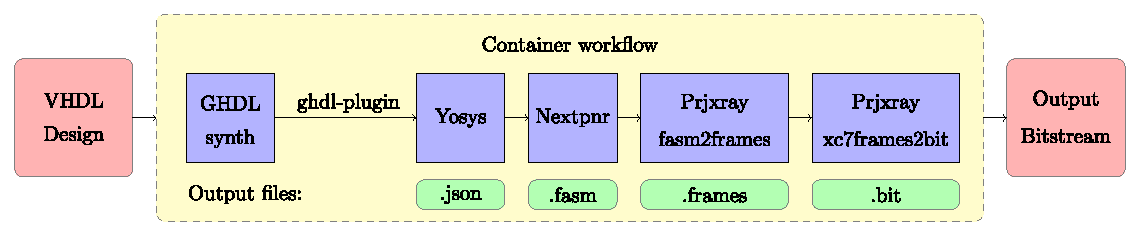
\includegraphics[width=151mm]{figures/container_workflow.pdf}
    \caption{Container workflow to generate bitstream from VHDL code.}
    \label{fig:workf}
\end{figure}

\subsection{Shell/Bash script}

\label{shell:script}

This container has the necessary FLOS tools installed inside it to generate bitstreams from your VHDL code. 
However, to automate the bitstream generation process, you can generate a shell/bash script \textit{(.sh)}.
This script will be executed inside the container and will perform all the steps to generate the bitstream using the internal FLOS tools installed in it.

\vspace{5mm}

\noindent The point is to facilitate the use of the container, in this order with a single command you will open a container from the downloaded image, run the shell/bash script inside this container, generate the bitstream from the VHDL sources and close the container simplifying the execution of the workflow.
In the section \ref{run} is specify how this script looks like.

\vspace{5mm}

\noindent To generate the bitstream from your VHDL code you must consider the relative paths that the shell/bash script points. 
In this context, if you run the container in the directory where your sources are, you must refers in the description of the script this paths.
More specifically, the part of the shell/bash code whose compile the VHDL code with GHDL must have the correct paths to include the sources and perform the compilation correctly.

\vspace{5mm}

\noindent To execute the sheel/bash script through the container you must add the argument \ref{cod:1} to open a shell inside it and execute your script. 
With this command you can execute several commands inside the open terminal by concatenating them through \textit{\&\&} symbol. 
For example, if you want to set a environment variable and then execute your script you can run \say{\mintinline[breaklines]{bash}{EnvVariable=YOUR_envVARIABLE && ./your_bash_script.sh}}.

\begin{code}
%\begin{minted}[frame=lines,framesep=2mm,baselinestretch=1.2,fontsize=\footnotesize,breaklines,linenos]{bash}
\begin{minted}[frame=lines,framesep=2mm,baselinestretch=1.2,fontsize=\footnotesize,breaklines]{bash}
                            sh -c "task1 && task2 && ..."
\end{minted}
\caption{Argument to add to the run container command to open a terminal inside it.}
\label{cod:1}
\end{code}

\vspace{5mm}

\noindent In conclusion, in order to operate in an easy and simplified way with the container you will open it, execute the workflow through the shell/bash script to generate the bitstream from your VHDL code and immediately close the container, all the execution through a single command \ref{cod:3}.
Instead of opening the container, locating you inside it and execute the workflow point by point.

\subsubsection{Shebang}

\label{shebang}

The shebang is a piece of code that indicates the path of the program that will interpret the script.
In this case, the interpreter is going to be bash.
Therefore, at the beginning of the script, you will indicate it through the piece of code \ref{cod:2}.

\vspace{10mm}

\begin{code}
\begin{minted}[frame=lines,framesep=2mm,baselinestretch=1.2,fontsize=\footnotesize,breaklines]{bash}
                                #!/usr/bin/env bash
\end{minted}
\caption{Shebang to interpret the script with bash.}
\label{cod:2}
\end{code}


\subsection{Container management tool}

In order to management the containers you must have a tool. 
Principally, there are two tools to perform this management: Podman \cite{podman} \cite{gh:podman} and Docker \cite{docker} \cite{gh:docker} \cite{gh:moby}.

\vspace{5mm}

\noindent In this case Podman is used, but for the Docker case it is basically the same.
First, you are going to download/install the tool aplliying the following commands depending your Linux distro:

\begin{itemize}
\item Fedora: \mintinline[breaklines]{bash}{sudo dnf -y install podman}
\item Debian: \mintinline[breaklines]{bash}{sudo apt-get -y install podman}
\item Arch Linux \& Manjaro Linux: \mintinline[breaklines]{bash}{sudo pacman -S podman}
\item Gentoo: \mintinline[breaklines]{bash}{sudo emerge app-containers/podman}
\end{itemize}

\noindent It is suggested that the users of this guide learn more about the containers, their use, how they work and how they are built, since in this UG only the couple of commands to operate this particular container \cite{gh:container-implarty} will be mentioned.

\vspace{5mm}

\noindent These commands are:

\begin{enumerate}
\item \mintinline[breaklines]{bash}{podman pull ghcr.io/unike267/containers/impl-arty:latest}
    \begin{itemize}
    \item To download the image. 
    \item \textit{ghcr.io} refers to the container is hosted on GitHub.
    \item To use this command in Docker remplace \say{podman} with \say{docker}. 
    \end{itemize}
\item \mintinline[breaklines]{bash}{podman images}
    \begin{itemize}
    \item To view downloaded images.
    \item In this context, it will appear:
        \begin{itemize}
        \item \mintinline[breaklines]{bash}{ghcr.io/unike267/containers/impl-arty   latest  IMAGE ID}  \mintinline[breaklines]{bash}{      CREATED DATA    SIZE}
        \end{itemize}
    \item To use this command in Docker remplace \say{podman} with \say{docker}. 
    \end{itemize}
\item\label{cod:3} \mintinline[breaklines]{bash}{podman run --rm -itv $(pwd):/wrk:Z -w /wrk unike267/containers/impl-arty sh -c "shell/bash tasks"} 
    \begin{itemize}
    \item To run the container. 
    \item In this context, the arguments are used for the following \cite{podman:run}:
        \begin{itemize}
        \item[>] \mintinline[breaklines]{bash}{--rm}: To remove the container when the command is finished, i.e. when the shell tasks are finished.
        \item[>] \mintinline[breaklines]{bash}{-itv} \footnote{According to the POSIX standard \cite{posix} \cite{posix:wiki}, applying \mintinline[breaklines]{bash}{-itv} is the same as applying \mintinline[breaklines]{bash}{-i -t -v}, unlike using two dashes as in the case of \mintinline[breaklines]{bash}{--rm} which means only \say{remove}. 
That is, when a single dash is used each letter is an argument and several arguments can be linked, when two dashes are used all letters are part of the same argument.}:
            \begin{itemize}
                \item[>] \mintinline[breaklines]{bash}{-i} (interactive): To indicate that whatever you write gets into the container.
                \item[>] \mintinline[breaklines]{bash}{-t} (\mintinline[breaklines]{bash}{--tty} Allocate a pseudo-TTY): To tell the container that the execution is being performed from a target that has a screen and keyboard, so it makes sense to print things like logs.
                \item[>] \mintinline[breaklines]{bash}{-v} (volume): To create a bind mount through the following scheme: {\fontsize{9.5}{30}\selectfont [[SOURCE-VOLUME|HOST-DIR:]CONTAINER-DIR[:OPTIONS]]}. 
In this case the scheme takes the form \mintinline[breaklines]{bash}{(pwd):/wrk:Z}, which means that the host directory is the directory where the run command is executed, the container directory is \mintinline[breaklines]{bash}{/wrk} and the option \mintinline[breaklines]{bash}{:Z} tells Podman the label of the container content.
            \end{itemize}
        \item[>] \mintinline[breaklines]{bash}{-w} (work directory): to indicate the working directory inside the container, in this case this directory is \mintinline[breaklines]{bash}{/wrk}.
        \item[>] \mintinline[breaklines]{bash}{unike267/containers/impl-arty}: is the image from which the container will be launched.
        \item[>] \mintinline[breaklines]{bash}{sh -c "shell/bash tasks"}: is explained in subsection \ref{shell:script}.
        \end{itemize}
    \item To use this command in Docker remplace \say{podman} with \say{docker}. 
    \end{itemize}
\item \mintinline[breaklines]{bash}{podman ps -a}
    \begin{itemize}
    \item To check which containers are open.
    \item In this context, there shouldn't be any open container because the container is closed when the script is executed.
    \item To use this command in Docker remplace \say{podman} with \say{docker}. 
    \end{itemize}
\end{enumerate}

\noindent At the moment, these 4 commands are the only thing you need to know about containers and executing the third one \ref{cod:3} is enough to generate bitstreams from your VHDL code through FLOS tools.


\section{Example: run the container}

\label{run}

Now the basic concepts of the \ref{intro} section are going to be applied to generate the NEORV32 RISC-V soft-core bitstream for the Arty A7 35T and 100T from the VHDL code available in the following repository \cite{gh:neorv32} \cite{gh:neorv32-setups}.

\vspace{5mm}

\noindent This example is uploaded and run in CI in the following branch \href{https://github.com/Unike267/Containers/tree/neorv32-setups}{gh:Unike267 /Containers/tree/neorv32-setups}.
The script that is used in this example is as follows:

\begin{code}
\begin{minted}[frame=lines,framesep=2mm,baselinestretch=1.2,fontsize=\footnotesize,breaklines,linenos]{bash}
#!/usr/bin/env bash

set -ex

cd $(dirname "$0")

if [[ -z "${Board}" ]]; then
  Arty='35t'
elif [[ $Board == '35t' ]]; then
  Arty='35t'
elif [[ $Board == '100t' ]]; then
  Arty='100t'
else
  echo "Error Board must be 35t or 100t"
  exit
fi

echo "Selected board is" $Arty

apt update -qq

apt install -y git

git clone --recursive https://github.com/stnolting/neorv32-setups

mkdir -p build

echo "Analyze NEORV32 CPU"

ghdl -i --workdir=build --work=neorv32  ./neorv32-setups/neorv32/rtl/core/*.vhd
ghdl -i --workdir=build --work=neorv32 ./neorv32-setups/neorv32/rtl/test_setups/neorv32_test_setup_bootloader.vhd
ghdl -m --workdir=build --work=neorv32 neorv32_test_setup_bootloader

echo "Synthesis with yosys and ghdl as module"

yosys -m ghdl -p 'ghdl --workdir=build --work=neorv32 neorv32_test_setup_bootloader; synth_xilinx -nodsp -nolutram -flatten -abc9 -arch xc7 -top neorv32_test_setup_bootloader; write_json neorv32_test_setup_bootloader.json' 

if [[ $Arty == '35t' ]]; then
  echo "Place and route"
  nextpnr-xilinx --chipdb /usr/local/share/nextpnr/xilinx-chipdb/xc7a35t.bin --xdc arty.xdc --json neorv32_test_setup_bootloader.json --write neorv32_test_setup_bootloader_routed.json --fasm neorv32_test_setup_bootloader.fasm
  echo "Generate bitstream"
  ../../prjxray/utils/fasm2frames.py --part xc7a35tcsg324-1 --db-root /usr/local/share/nextpnr/prjxray-db/artix7 neorv32_test_setup_bootloader.fasm > neorv32_test_setup_bootloader.frames
  ../../prjxray/build/tools/xc7frames2bit --part_file /usr/local/share/nextpnr/prjxray-db/artix7/xc7a35tcsg324-1/part.yaml --part_name xc7a35tcsg324-1 --frm_file neorv32_test_setup_bootloader.frames --output_file neorv32_test_setup_bootloader_35t.bit
elif [[ $Arty == '100t' ]]; then
  echo "Place and route"
  nextpnr-xilinx --chipdb /usr/local/share/nextpnr/xilinx-chipdb/xc7a100t.bin --xdc arty.xdc --json neorv32_test_setup_bootloader.json --write neorv32_test_setup_bootloader_routed.json --fasm neorv32_test_setup_bootloader.fasm
  echo "Generate bitstream"
  ../../prjxray/utils/fasm2frames.py --part xc7a100tcsg324-1 --db-root /usr/local/share/nextpnr/prjxray-db/artix7 neorv32_test_setup_bootloader.fasm > neorv32_test_setup_bootloader.frames
  ../../prjxray/build/tools/xc7frames2bit --part_file /usr/local/share/nextpnr/prjxray-db/artix7/xc7a100tcsg324-1/part.yaml --part_name xc7a100tcsg324-1 --frm_file neorv32_test_setup_bootloader.frames --output_file neorv32_test_setup_bootloader_100t.bit
fi

echo "Implementation completed"
\end{minted}
\caption{The shell/bash script to generate NEORV32 bistream from its VHDL code.}
\label{cod:4}
\end{code}

\vspace{5mm}

\noindent Each piece of this script is explained in the following subsections.

\subsection{Intro \& set board: from line 1 to line 18}

The first line is the shebang, this concept is explained in \ref{shebang}.

\vspace{5mm}

\noindent The third line, \mintinline[breaklines]{bash}{set -ex}, is the conbination of \mintinline[breaklines]{bash}{set -e} and \mintinline[breaklines]{bash}{set -x}. 
The first one indicates to exit the script as soon as any line in the bash script fails. The second one prints each command that is going to be executed with a little plus.

\vspace{5mm}

\noindent The fifth line, \mintinline[breaklines]{bash}{cd $(dirname "$0")}, identifies and locates in the directory that contains the script (which might be different than the current working directory). 
Suppose your script is /home/wherever/your\_script.sh. In this context, \mintinline[breaklines]{bash}{$0} is your\_script.sh, \mintinline[breaklines]{bash}{$(dirname "$0")} is /home/wherever/ and  \mintinline[breaklines]{bash}{cd} command is located in that path.

\vspace{5mm}

\noindent From line 7 to line 16 the environment variable \say{Board} is introduced in the local variable \say{Arty}.
If the environment variable would not exist \mintinline[breaklines]{bash}{[-z "${Board}"]}, the Arty variable would be set to 35t.

\vspace{5mm}

\noindent Line 18 just displays the value of the local variable \say{Arty}.

\subsection{Download NEORV32 sources: from line 20 to line 24}

\label{ci:lines}

Ignore this step if you are going to use your own VHDL code.

\vspace{5mm}

\noindent If your are going to follow this example (implementation of NEORV32) but you are performing it in local and you have GIT insatalled, ignore line 20 and line 22. 
This lines are thought to perform the example through Continous Integration (CI).

\vspace{5mm}

\noindent Line 24 downloads the \say{neorv32-setups} repository  from GitHub. 
This repository has the \say{neorv32} repository as a submodule, so the argument \mintinline[breaklines]{bash}{--recursive} is used to add it.

\subsection{VHDL compilation through GHDL: from line 26 to line 32}

Line 26 creates a directory named \say{build} to store in it the compilation output files. The \mintinline[breaklines]{bash}{-p} argument means \say{parents} and it uses to create a directory with top-down approach. 
That is, it offers the possibility of creating a directory inside another directory inside another etc (\mintinline[breaklines]{bash}{mkdir -p main/within_main}). 
In this example only one directory is created so the \mintinline[breaklines]{bash}{-p} argument is not strictly necessary.

\vspace{5mm}

\noindent Line 28 displays the sentence within \mintinline[breaklines]{bash}{""}.

\vspace{5mm} 

\noindent Line 30 and 31 import the VHDL code through \mintinline[breaklines]{bash}{-i} argument. 
In this context, \mintinline[breaklines]{bash}{--workdir} argument indicates the working directory where the output files will be stored and \mintinline[breaklines]{bash}{--work} argument indicates the \say{neorv32} library. 
It should be noted that if you want to use VHDL 2008 standard you must add after \mintinline[breaklines]{bash}{-i} argument \mintinline[breaklines]{bash}{--std=08}.

\vspace{5mm} 

\noindent Line 32 performs the compilation through the argument make (\mintinline[breaklines]{bash}{-m}). 
In this context, the top of the design must be indicated, in this case is \say{neorv32\_test\_setup \_bootloader}.
In addition, the working directory and the library \say{neorv32} are set.

\subsection{Synthesis with Yosys and GHDL as module: from line 34 to line 36}

Line 34 displays the sentence within \mintinline[breaklines]{bash}{""}.

\vspace{5mm} 

\noindent Line 36 performs the synthesis through Yosys with GHDL as module. In this context, \mintinline[breaklines]{bash}{-m} argument load the specified \say{plugin} module, in this case \say{ghdl-yosys-plugin}. 
Then, \mintinline[breaklines]{bash}{-p} argument execute the commands within \mintinline[breaklines]{bash}{''}.
These commands are separated by \mintinline[breaklines]{bash}{;} forming three steps. 

\vspace{5mm} 

\noindent The first step is to perform the synthesis with GHDL (\mintinline[breaklines]{bash}{--synth}), consequently the working directory and the library \say{neorv32} are set.

\vspace{5mm} 

\noindent The second step is to perform the synthesis for Xilinx 7-Series FPGAs. This is indicated by \mintinline[breaklines]{bash}{synth_xilinx}. 
In this context, you must disable the implementation using DSPs and distributed ram (LUT RAM).
Since at the moment, Yosys doesn't support the mapping of these elements for Xilinix architectures, see \ref{limit} section. 
The argument \mintinline[breaklines]{bash}{-flatten} flattens the design by replacing cells by their implementation. The argument \mintinline[breaklines]{bash}{-abc9} is to set ABC9 for technology mapping. 
The argument \mintinline[breaklines]{bash}{-xc7} generates the synthesis netlist for the xc7 architecture family.
The argument \mintinline[breaklines]{bash}{-top} indicates the top of the design.

\vspace{5mm} 

\noindent The third step write a JSON netlist of the current design named \say{neorv32\_test\_ setup\_bootloader.json}.

\subsection{Perform P\&R and generate bitstrem for Arty A7 35t board: from line 38 to line 43}

Line 38 select the task to perform P\&R and generate bitstrem for Arty A7 35t.

\vspace{5mm} 

\noindent Line 39 displays the sentence within \mintinline[breaklines]{bash}{""}.

\vspace{5mm} 

\noindent Line 40 performs P\&R through Nextpnr-Xilinx. 
In this context, the argument \mintinline[breaklines]{bash}{--chipdb} select the chip data base, in this case the one related to the Arty 35t.
Then, the .xcd file named \say{arty.xdc} is imported. \footnote{The sintaxys of the .xdc file is slightly different from the one supported by vivado, see the .xdc file of the example.} 
Also, the yosys output JSON file is imported.
Finally, the output routed files are written, in this case in JSON and FASM format. 

\vspace{5mm} 

\noindent Line 41 displays the sentence within \mintinline[breaklines]{bash}{""}.

\vspace{5mm} 

\noindent Lines 42 and 43 use the Python programs of the Project X-Ray to generate the bitstream from Nextpnr-Xilinx output FASM file.

\subsection{Perform P\&R and generate bitstrem for Arty A7 100t board: from line 44 to line 50}

Line 44 select the task to perform P\&R and generate bitstrem for Arty A7 100t.

\vspace{5mm} 

\noindent Line 45 displays the sentence within \mintinline[breaklines]{bash}{""}.

\vspace{5mm} 

\noindent Line 46 performs P\&R through Nextpnr-Xilinx. 
In this context, the argument \mintinline[breaklines]{bash}{--chipdb} select the chip data base, in this case the one related to the Arty 100t.
Then, the .xcd file named \say{arty.xdc} is imported.
Also, the yosys output JSON file is imported. \footnote{The yosys output JSON file is the same for both boards.}
Finally, the output routed files are written, in this case in JSON and FASM format. 

\vspace{5mm} 

\noindent Line 47 displays the sentence within \mintinline[breaklines]{bash}{""}.

\vspace{5mm} 

\noindent Lines 48 and 49 use the Python programs of the Project X-Ray to generate the bitstream from Nextpnr-Xilinx output FASM file.

\subsection{Commands to generate bitstream through the container.}

To generate the bitstream through the container just apply code \ref{cod:5} for the Arty A7 35t and code \ref{cod:6} for the Arty A7 100t. 
In this context, the \say{script.h} for the case of the example is the code \ref{cod:4}.

\vspace{5mm} 

\noindent Remember, if you run this command locally, ignore the corresponding lines according to subsection \ref{ci:lines}.

\begin{code}
\begin{minted}[frame=lines,framesep=2mm,baselinestretch=1.2,fontsize=\footnotesize,breaklines]{bash}
podman run --rm -itv $(pwd):/wrk:Z -w /wrk unike267/containers/impl-arty sh -c "Board=35t && script.sh"
\end{minted}
\caption{Command to generate bitstream for the Arty A7 35t.}
\label{cod:5}
\end{code}

\begin{code}
\begin{minted}[frame=lines,framesep=2mm,baselinestretch=1.2,fontsize=\footnotesize,breaklines]{bash}
podman run --rm -itv $(pwd):/wrk:Z -w /wrk unike267/containers/impl-arty sh -c "Board=100t && script.sh"
\end{minted}
\caption{Command to generate bitstream for the Arty A7 100t.}
\label{cod:6}
\end{code}

\vspace{15mm} 


\section{Limitations of the FLOS tools that integrate the container}

\label{limit}

First, it should be noted that functional bitstreams of the SoC have been achieved using this container for the Arty A7 35T and 100T FPGAs.

\vspace{5mm} 

\noindent However, the generation of the bitstream through these FLOS tools have a couple of limitations:

\begin{itemize}
\item Yosys synthesis, in the case of Xilinx, does not support an implementation using DSPs or distributed RAM (LUT RAM).
Just as for Lattice this tool is very mature, for Xilinx this tool is at an early stage.
\vspace{2mm}
\item In case NEORV32 is synthesized with its own \say{app\_image}, without using the bootloader (in the example the bootloader is used), the IMEM implementation is limited (I use 6*1024 bits). Therefore, the size of the compiled programs is restricted.
If a large IMEM is implemented, which in Vivado would be supported, the generated bitstream does not work.
\end{itemize}

\section{Implementation the workflow through CI}

\label{ci}

To generate bitstream through FLOS tools in GitHub Continous Integration (CI) you can use the following YML file:

\begin{code}
\begin{minted}[frame=lines,framesep=2mm,baselinestretch=1.2,fontsize=\footnotesize,breaklines,linenos]{yaml}
name: neorv32_impl

on:
  push:

jobs:

  neorv32_impl_35t:
    runs-on: ubuntu-latest
    env:
      Board: 35t

    steps:

      - name: 'Checkout'
        uses: actions/checkout@v4

      - uses: docker://ghcr.io/unike267/containers/impl-arty:latest
        with:
          args: ./test.sh
      
      - name: 'Upload artifact'
        uses: actions/upload-artifact@v4
        with:
          name: neorv32_impl_35t
          path: ./neorv32_test_setup_bootloader_35t.bit

  neorv32_impl_100t:
    runs-on: ubuntu-latest
    env:
      Board: 100t

    steps:

      - name: 'Checkout'
        uses: actions/checkout@v4

      - uses: docker://ghcr.io/unike267/containers/impl-arty:latest
        with:
          args: ./test.sh
      
      - name: 'Upload artifact'
        uses: actions/upload-artifact@v4
        with:
          name: neorv32_impl_100t
          path: ./neorv32_test_setup_bootloader_100t.bit
\end{minted}
\caption{YML file to generate bitstream through FLOS tools in CI.}
\label{cod:7}
\end{code}

\vspace{3mm}

\noindent Lines 10-11 and 30-31 set the environment variable.

\vspace{3mm}

\noindent Lines 18 and 38 set the container.

\vspace{3mm}

\noindent Lines 20 and 40 run the script through the container.

\vspace{3mm}

\noindent Lines 22-23-24-25-26 and 42-43-44-45-46 upload the bitstream as an artifact.



\clearpage % If you want the references in a separate page
\bibliography{bibliography}

%\clearpage % If you want the appendix in a separate page
%\appendix
%\input{sections/appendix}

\end{document}

